\section{Overall description}
\subsection{Product perspective}
	\subsubsection{System interfaces}
	\label{sec:systemInterfaces}
		The system we are to develop will have some external interfaces (represented in \autoref{fig:systemInterfaces}) to accomplish the \hyperref[sec:goals]{goals stated before}.
		\begin{figure}[h]
			\centering
			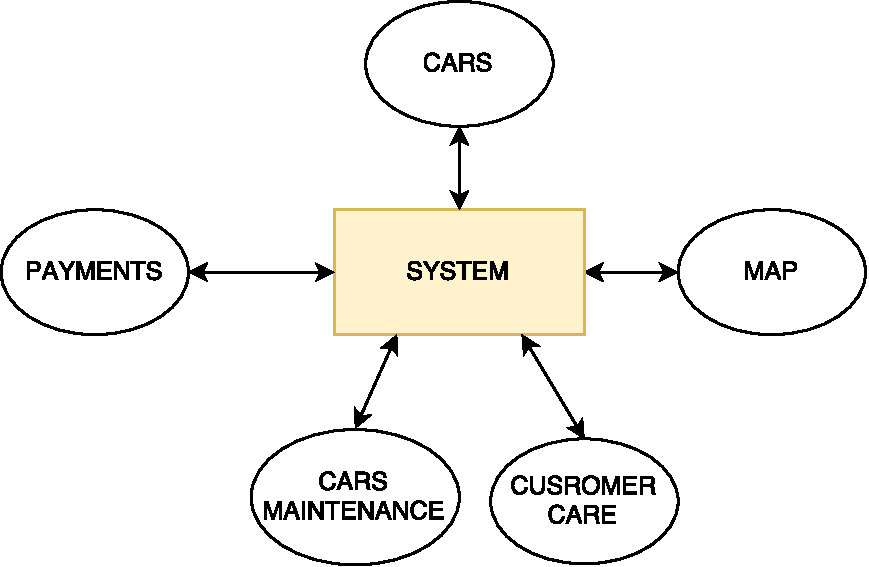
\includegraphics[scale=0.5]{system_blocks}
			\caption{
				\label{fig:systemInterfaces} 
				Overview of system interfaces
			}
		\end{figure}
	\paragraph{Payments}
	When a payment is required (e.g. when a user ends his rent) the system sends a request with all the details needed to complete the payment (i.d. name and surname of the user, due amount, credit card number etc.) to an external payment handling system. Once the external system completes the payment process, it sends our system the payment outcome so that the system can take appropriate action.
	
	\paragraph{Customer care} Every time it is required, a PowerEnJoy customer care service operator can interact with a user. Customer care service operators can request and see all user details, their rents and payments history. Such operators can also mark or unmark users as banned from the system, mark cars as not available and, in general, provide assistance to users.

	\paragraph{Maintenance} The system will interact with a preexisting car maintenance service which already deals with other car sharing services. Our system will expose to the maintenance service a real time list of all the cars tagged as \emph{not available} via a \emph{restricted access API} which will also provides their GPS position and a brief description of their problems. The maintenance service takes care of reaching those cars, unlocks the doors, fixes the fault, locks the doors back and finally tags them as \emph{available} using the aforementioned API provided by the system. See \hyperref[sec:cars]{cars section} for more details.
	
	\paragraph{Map} GPS position of cars and safe areas is displayed to all users, customer care operators and maintenance operators on a constantly updated map which relies on an external GIS.

	\paragraph{Cars}\label{sec:cars}All cars provided by the customer are equipped with a communication system which ensures a continuous protected communication between the car and the system. All cars also have a module which provides a set of primitives that allow the system to retrieve information and to run commands to take actions on the car. A built-in user interface embedded with the modules shows some relevant information to the user.\\
	Information retrieved by the system from the car include:
	\begin{itemize}
		\item unique car identifier
		\item GPS position
		\item engine status (on, off)
		\item current number of passengers
		\item maximum number of passengers
		\item battery level (percentage)
		\item charging status (in charge, not in charge)
		\item door locking status (locked, unlocked)
		\item door closing status (open, closed)
	\end{itemize}
	For each of these information the car provides a primitive to instantiate a listener which triggers a notification to the system whenever the observed parameter changes.\\
\newline
	Information sent to the car by the system include:
	\begin{itemize}
		\item location of safe areas
		\item position of charging stations
		\item current time
		\item rent cost per hour
	\end{itemize}
	Commands runnable by the system include:
	\begin{itemize}
		\item lock doors
		\item unlock doors
		\item start rent timer
	\end{itemize}		
	Information shown to the user by the embedded car interface include:
	\begin{itemize}
		\item current car position (also w.r.t. safe areas and charging stations)
		\item number of passengers
		\item battery level (percentage)
		\item current time
		\item rent time
		\item amount owed until now (based upon rent cost per hour)
	\end{itemize}
	
	This system provides, among other functionalities, a secure way to unlock and lock the doors of the car: it has a command which returns a software key which can be sent to the maintenance operators; they are able to unlock and lock the car with a smartphone client  of the car's embedded system and the key.\\
	
	In order to determine which cars are in charge in which charging station the system checks if the charging status of a car is set to \emph{true} and its position is within a small distance from the charging station position.\\
	
	The maximum number of passengers represents the maximum number of passengers that were detected by the car during its last ride (defined as the last period from engine on to engine off).\\
		
\subsubsection{User interfaces}
	Using the interfaces of the system users can:
	\begin{enumerate}
		\item Register and log-in to the system
		\item On the map they can view the position of
			\begin{enumerate}[label=\alph*)]
				\item themselves
				\item safe areas
				\item available cars (with their current battery level)
				\item charging stations
			\end{enumerate}
		\item Reserve a car
		\item View customer care contacts 
		\item Unlock the reserved car
		\item View and edit personal information
		\item View rents and payments history
	\end{enumerate}

\subsubsection{Software interfaces}
Databases and DBMSs are clearly required in order to store data about users, cars, charging stations, safe areas etc.

As mentioned before (see \hyperref[sec:systemInterfaces]{system interfaces section}) the system needs to use external APIs and to expose interfaces in order to interact with other systems.

All vehicles have an embedded external software system, which is able to display all information described in \hyperref[sec:cars]{cars section}.

\subsection{User characteristics}
	Users can use our system when they want to rent a car.\\
	Necessary conditions for the user in order to use the system are:
	\begin{itemize}
		\item He must have a smartphone and be able to use it
		\item He must be in the age of majority
		\item He must have a proper valid driving license
		\item He must be able to drive a car (i.d. he must be in both physical and mental health)
	\end{itemize}
	The user agrees to these conditions during the registration to the system.

\subsection{Domain assumption}
	We assume that these assumptions hold true in the domain of our system 
	\begin{enumerate}[label=\textbf{DA\arabic*}]
		\item GPS position is supposed to be accurate (max error $\pm5$m)
		\item GPS position of all cars is always obtainable
		\item The user who reserves the car will always be the person who drives it
		\item Users are legally allowed to drive cars (i.d. users have a proper driving license)
		\item Charging stations are always working correctly
		\item All data provided by users are correct and reliable
		\item All cars provided by the customer are equipped with a module which provides a set of
		primitives that allow the system to retrieve all the information it needs about
		the car and to run commands which allow the system to take actions on the car. See \hyperref[sec:cars]{cars section} for more details.
		\item Charging station can exclusively be used by PowerEnJoy cars
		\item The set of safe areas is pre-defined and is provided to our system by the customer
		\item The position of charging station is provided to our system by the customer
		\item All charging station are located inside safe areas
		\item The maps provided by the GIS are always up to date
		\item The commands sent to cars by the system are always executed
		correctly
		\item Information provided by the car are always correct and reliable
		\item Position of the user is always available when he uses our system
		
	\end{enumerate}
	
\clearpage
\subsection{The World and the Machine}
The world and the machine is a way of thinking about problems and phenomena relevant in the reality of the software system we are to develop. The world contains the phenomena that happens in reality but are not observable by our system; the machine instead contains the phenomena which take place inside the system and are not observable from outside of it. The intersection between these two sets of phenomena is the so called set of shared phenomena, which contains the phenomena that are controlled by the world and observed by the machine or controlled by the machine and observed by the world.
\newline
\\
Goals are prescriptive assertions formulated in terms of world phenomena (not necessarily shared); domain properties/assumptions are descriptive assertions assumed to hold in the world; requirements are prescriptive assertions formulated in terms of shared phenomena.\cite{WorldMachine}
\\
\\

\begin{figure}[h!]
	\centering
	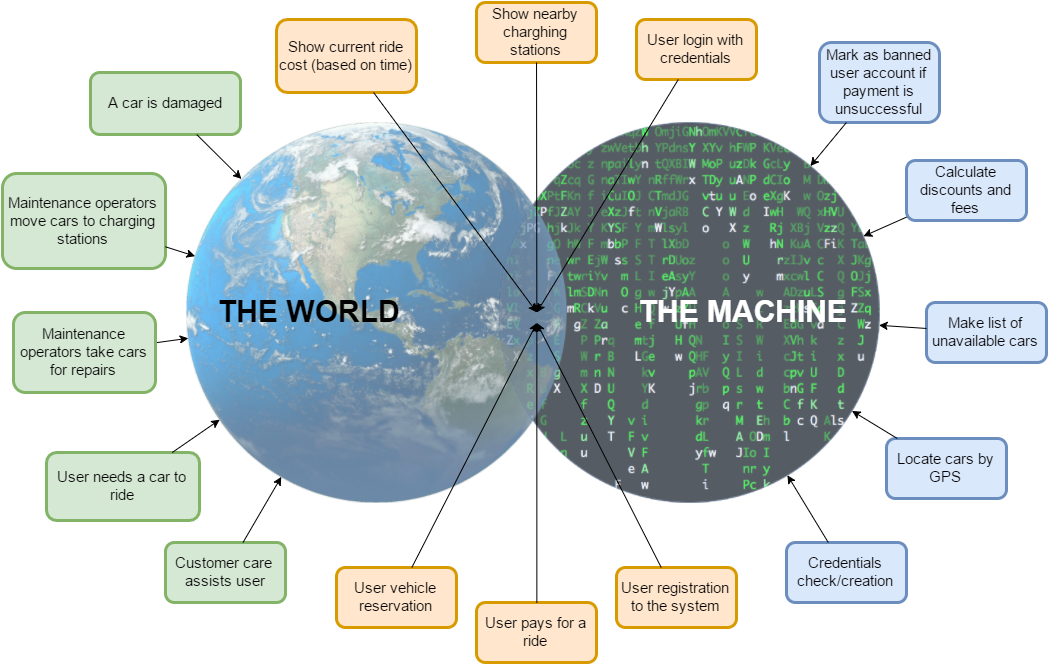
\includegraphics [width=\textwidth]{TheWorldAndTheMachine}
	\caption{
		\label{fig:WorldandMachine} 
		The World and the Machine
	}
\end{figure}
\clearpage